\refstepcounter{figure}
\noindent Figure \thefigure\ shows energy consumption.

\begin{center}
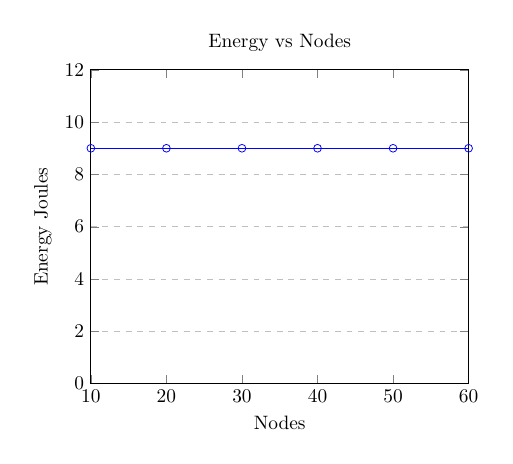
\begin{tikzpicture}[scale=0.7]
\begin{axis}[
title={Energy vs Nodes},
xlabel={Nodes}, ylabel={Energy Joules},
xmin=10, xmax=60, ymin=0, ymax=12,
xtick={10,20,30,40,50,60},
ymajorgrids=true, grid style=dashed,
]

\addplot[color=blue, mark=o] coordinates {(10,9) (20,9) (30,9) (40,9) (50,9) (60,9)};

\end{axis}
\end{tikzpicture}

\textbf{Figure \thefigure: Energy vs Nodes}
\label{fig:energy_density}
\end{center}